\chapter{プロセス同期}
\label{synchronaization}
これまで見てきたように,
複数のプロセス(スレッド)が並行して実行される.
複数の並行して実行されるプロセス(スレッド)が,決して競合することなく,
必要に応じて協調して動作するために,プロセス(スレッド)間で同期をとる必要がある.
この章ではプロセス(スレッド)間の同期について勉強する.

%==============================================================================
\section{競合(Race Condition, Competition)}
複数のプロセス(スレッド)が資源を共有して処理を進めることがある.
ここで言う資源とは
「スレッド間で共有する変数」,
「プロセス間で共有するメモリ」,
「カーネル内部のデータ構造」,
「ファイル」,
「入出力装置」
等が考えられる.
共有する資源をプロセス(スレッド)がアクセスする時,
きちんとした取り決めが無いと誤った結果になる場合がある.

例えば,銀行口座を管理する架空の例を考えてみよう.
一つのプロセス内で,入金を処理するスレッドと,
引き落としを処理するスレッドが並行して実行されているとする.
\figref{race}に,このプロセスの処理内容の一部をTeC風のアセンブリ言語で示す.
プロセスがほぼ同時に,
給料3万円の振込とカード料金2万円の引き落としを受信したとする.
二つのスレッドが競って\|account|変数の更新をする.
処理前は\|account|変数に口座の残高10万円が記録されていたとする.

\begin{myfig}{btp}{共有変数をアクセスする二つのスレッド}{race}
  \lstinputlisting[numbers=none]{Lst/race.txt}
\end{myfig}

\begin{quote}
  \begin{enumerate}
  \item (1)→(2)→(3)→(a)→(b)→(c)の順で実行された場合 \\
    \|account|変数の値は11万円になり正しい結果になる.

  \item (a)→(b)→(c)→(1)→(2)→(3)の順で実行された場合 \\
    \|account|変数の値は11万円になり正しい結果になる.

  \item (1)→(2)→(a)→(b)→(c)→(3)の順で実行された場合 \\
    入金管理スレッドが途中でpreemptionし,
    引き落としスレッドが実行された後,
    入金管理スレッドが再開された場合である.
    \|account|変数の値は13万円になる.

  \item (1)→(a)→(2)→(b)→(3)→(c)の順で実行された場合 \\
    二つのCPUが並列にスレッドを実行した場合である.
    \|account|変数の値は8万円になる.
  \end{enumerate}
\end{quote}

以上のように,
スレッドの実行順序等により計算結果が間違ってしまうことがある.
これは資源の利用について,
\emph{競合}(\emph{Race Condition} または \emph{Competition})が
発生しているからである.

%==============================================================================
\section{クリティカルセクション(Critical Section)}
\label{criticalsection}
競合が発生するのは,
一方のスレッドが自分のCPUレジスタにコピーした\|account|の値を
変更し書き戻すまでの間(変更中)に,
もう一方のスレッドが\|account|の値を
自分のCPUレジスタにコピーすることが原因である.
「変更中」の共有変数に他のスレッドがアクセスすることを禁止する必要がある.
他のスレッドが共有変数にアクセスすることが許されないプログラムの区間を
\emph{クリティカルセクション(Critical Section)},または,
\emph{クリティカルリージョン(Critical Region)}と呼ぶ.

\figref{race}の例で「(1)から(3)」と「(a)から(c)」は
\|account|変数のクリティカルセクションであり,
この区間をどれかのスレッドが実行している間は,
他のスレッドが\|account|変数にアクセスしてはならない.
クリティカルセクションの競合問題を効率よく解決するためには,
次の三つの条件を満たす必要がある.

\begin{quote}
  \begin{enumerate}
  \item 二つ以上のプロセス(スレッド)が同時にクリティカルセクションに入らない.
  \item クリティカルセクションに入っているプロセス(スレッド)がない時は,
    待たされることなくクリティカルセクションに入ることができる.
  \item クリティカルセクションに入るために永遠に待たされることがない.
  \end{enumerate}
\end{quote}

%==============================================================================
\section{相互排除(Mutual Exclusion)}
複数のプロセス(スレッド)が同時にクリティカルセクションに
入らないように制御することである.
\emph{排他制御}または\emph{相互排他}とも呼ばれる.
\emph{相互排除}を達成するために,
プロセス(スレッド)は,
クリティカルセクションに入る際に権利を得る手続きを行う.
これを行うプログラムの部分を
\emph{エントリーセクション(Entry Section)}と呼ぶ.
クリティカルセクションを出る際に権利を返却する手続きを行う.
これを行うプログラムの部分を
\emph{エグジットセクション(Exit Section)}と呼ぶ.

\subsection{割込み禁止}
\label{disableInterrupt}
シングルプロセッサ(CPUが一つしかない)システムでは,
クリティカルセクションを実行するとき割込みを禁止することで目的を達成できる.
\figref{disableInterrupt}に\figref{race}を改良したプログラムを示す.

\begin{myfig}{btp}{割込み禁止による相互排除}{disableInterrupt}
  \lstinputlisting[numbers=none]{Lst/disableInterrupt.txt}
\end{myfig}

エントリーセクションで
DI(Disable Interrrupt)命令を実行し割込みを禁止する.
エグジットセクションで
EI(Enable Interrrupt)命令を実行し割込みを許可する.
クリティカルセクションでは,
CPUが割込みを受付けない\footnote{
  再度,割込みが許可されるまで保留になる.
  プリエンプションはクリティカルセクションを出るまで遅延する.
}のでプリエンプションは発生しない.
クリティカルセクションの終わりまでCPUは連続して命令を実行する.
また,CPUが一つしかないので,他のCPUが\|account|変数をアクセスこともない.
よって,\|account|変数の変更中に他のプロセス(スレッド)が
\|account|変数をアクセスすることはない.

この方法は簡単に相互排除を行うことができるが,
割込み禁止時間が長くならないように注意する必要がある.
割込み禁止が長くなると,
タイマーからの割込みを取りこぼし時計が正確に進まなくなったり,
入出力装置の制御が間に合わなくなるなどの弊害が生じる\footnote{
  割込み禁止期間に同じ割込みが複数回発生した場合,
  割込み許可になったとき割込みの種類につき一度だけ割込みが発生する.
  ハードウェアに,保留になった割込みのカウンタはない.}.
また,DI命令,EI命令は特権命令なので,
カーネル内だけで使用できる手法である.

\subsection{専用命令を用いる方式}
マルチプロセッサ(CPUが複数ある)システムでは,
割込み禁止による方法では目的を達成することができない.
クリティカルセクションでプリエンプションが発生しなくても,
他のCPUによって実行されるプロセス(スレッド)がクリティカルセクションに
入る可能性があるからである.

マルチプロセッサシステムとは,
\figref{hardBlock}に示したメモリを共有するSMPシステムのことである.
複数のCPUによるメモリのアクセスはハードウェアにより順序付けされる.
同じメモリアドレスへのアクセスが競合し,
どちらのCPUが書き込んだ値とも異なる値になることはない.
順序付けの結果,後になった書き込みの結果がメモリに残る.
また機械語命令は,一部の例外を除いて,
途中で割込まれることはない.
このようなシステムでは,
以下の機械語命令を相互排除の目的に使用できる.

\begin{itemize}
\item \emph{TS(Test and Set)命令} \\
  TS命令は「(1) メモリの値をCPUレジスタにロード」し,
  「(2) 1を同じメモリアドレスに書き込む」命令である.
  この二つを他のCPUのメモリアクセスに割込まれることなく,
  \emph{アトミック(atomic)}に実行する.
  TS命令(\|TS R,M|)の動作は,例えば次のようになる.

  \begin{quote}
    \begin{enumerate}
    \item バスをロックする
    \item $R \leftarrow [M]$
    \item \texttt{if (R==0) } $Zero \leftarrow 1;$
      \texttt{~else} $Zero \leftarrow 0;$
    \item $[M] \leftarrow 1$
    \item バスのロックを解除する
    \end{enumerate}
  \end{quote}

  まず,他のCPUがメモリをアクセスしないようにバスをロックする.
  次に,メモリの指定番地から値をCPUレジスタにロードする.
  また,レジスタの値によってCPUの$Zero$フラグの値を決める.
  更に,メモリの指定番地に\texttt{1}をストアする.
  最後にバスのロックを解除する.
  ロードとストアで合計二回のメモリアクセスがあるが,
  バスがロックされているので,
  TS命令の実行途中に他のCPUがメモリをアクセスすることはない.
  \figref{testAndSet}にTS命令の使用例を示す.
  JZ命令は$Zero$フラグが\texttt{1}の場合のみジャンプする.
  この例のように,
  エントリーセクションでループして待つ方式を
  \emph{ビジーウェイティング(Busy Waiting)}と呼ぶ.

  \begin{myfig}{btp}{TS命令の使用例}{testAndSet}
    \lstinputlisting[numbers=none]{Lst/testAndSet.s}
  \end{myfig}

  メモリのクリアは通常のST命令でできる\footnote{
    通常の命令もメモリアクセスする度にバスをロックしている.}.
  TS命令を用いる場合でも,
  クリティカルセクションは割込み禁止で実行する必要がある.
  クリティカルセクションでのプリエンプションを避けるためである.
  もしも,優先度の低いプロセス(スレッド)が
  クリティカルセクション内でプリエンプションすると,
  優先度の高いプロセス(スレッド)が
  エントリーセクションで\emph{ビジーウェイティング}を始め
  \emph{デッドロック}に陥る可能性がある.
  この方式も,
  特権命令DI,EIを使用するのでカーネル内でしか利用できない.

\item \emph{SW(Swap)命令} \\
  SW(Swap)命令もSMPシステムでの相互排除に使用できる.
  「SW  R, M」は,以下を\emph{アトミック(atomic)}に実行する.

  \begin{quote}
    \begin{enumerate}
    \item バスをロックする
    \item $T \leftarrow [M]$
    \item $[M] \leftarrow R$
    \item $R \leftarrow T$
    \item バスのロックを解除する
    \end{enumerate}
  \end{quote}

  ここで $T$ はCPU内部の一時的なレジスタ
  ($T$ レジスタの存在はプログラムから見えない)である.
  \figref{swap}にSW命令の使用例を示す.
  使用例はTS命令のものと似ているので解説は省略する.

  \begin{myfig}{btp}{SW命令の使用例}{swap}
    \lstinputlisting[numbers=none]{Lst/swap.s}
  \end{myfig}

\item \emph{CAS(Compare And Swap)命令}\\
  CAS(Compare And Swap)命令もSMPシステムでの相互排除に使用できる.
  例えば「CAS  R0, R1, M」は,以下を\emph{アトミック(atomic)}に実行する.

  \begin{quote}
    \begin{enumerate}
    \item バスをロックする
    \item $T \leftarrow [M]$
    \item \texttt{if (T==R0) \{} $[M] \leftarrow R1;~ Zero \leftarrow 1;$
      \texttt{\} else \{} $R0 \leftarrow T;~  Zero \leftarrow 0;$ \texttt{\}}
    \item バスのロックを解除する
    \end{enumerate}
  \end{quote}

  CAS命令を用いたエントリーセクション,
  エグジットセクションの作り方も,
  TS命令と同様なのでここでは使用例を省略する.
  CAS命令を用いると共有資源にロックを掛けない,
  \emph{ロックフリー(Lock-free)}なアルゴリズムを実現できる.
  前出の銀行口座を管理する架空のプロセス(\figref{race})を
  CAS命令を用いて書換えた例を\figref{cas}に示す.

  \begin{myfig}{btp}{CAS命令を用いた口座管理プログラムの例}{cas}
    \lstinputlisting[numbers=none]{Lst/cas.txt}
  \end{myfig}

  処理開始時の\|account|の値をG1に保存しておく.
  計算結果を格納する際に,
  処理開始から\|account|の値が変化していないことを確認してから書き込む.
  以前の例では,
  他のプロセスが共有資源にアクセスしないように,
  何らかのロックを掛けていた.
  この方式はロックを掛けずに「結果を書き込む時点で判断」するので,
  ロックフリーなアルゴリズムである.
\end{itemize}

\subsection{フラグを用いる方式}
アルゴリズムを工夫しソフトウェアだけで相互排他を実現する方式である.
中でも1981年にG. L. Peterson が発表した
\emph{Petersonのアルゴリズム(Peterson's solution)}が有名なので紹介する.
\figref{peterson}にJava風の言語で書いた例を示す.

\begin{myfig}{btp}{Petersonのアルゴリズム}{peterson}
  \lstinputlisting[numbers=none]{Lst/peterson.txt}
\end{myfig}

このアルゴリズムの特徴は次の通りである.

\begin{quote}
  \begin{enumerate}
  \item マルチプロセッサシステムでも使用できる.
  \item 2プロセス(スレッド)以上に拡張可能だが複雑になる.
  \item 最近のプロセッサと相性が悪い.(out-of-order実行)
  \end{enumerate}
\end{quote}

%==============================================================================
\section{セマフォ(Semaphore)}
これまでに紹介してきた相互排除は,
主に\emph{ビジーウェイティング}を用いるものであり,
待っている間もCPUを使用し続ける.
また、割込み禁止にする必要があるのでカーネル内でしか使用できない.
これらは、カーネル内で短時間で終わる相互排除のために適しているが,
長時間に渡る場合やユーザプログラムが直接使用する場合には適さない.
そこで,オペレーティングシステムが提供するより洗練された
プロセス同期機構である\emph{セマフォ}を紹介する.
なお,これまでに紹介してきた相互排除は,セマフォを実現するためにも使用される.

\subsection{概要}
\emph{セマフォ(Semaphore:腕木式信号機)}は,
1965年に E. W. Dijkstra が提案したデータ型\footnote{
  C言語なら構造体を用いてセマフォ型を宣言する.
  \texttt{typedef struct \{ ... \} Semaphore;}
}である.
語源となった腕木式信号機は,
鉄道で使用される\figref{semaphore}のような信号機である.

\begin{myfig}{btp}{腕木式信号機}{semaphore}
  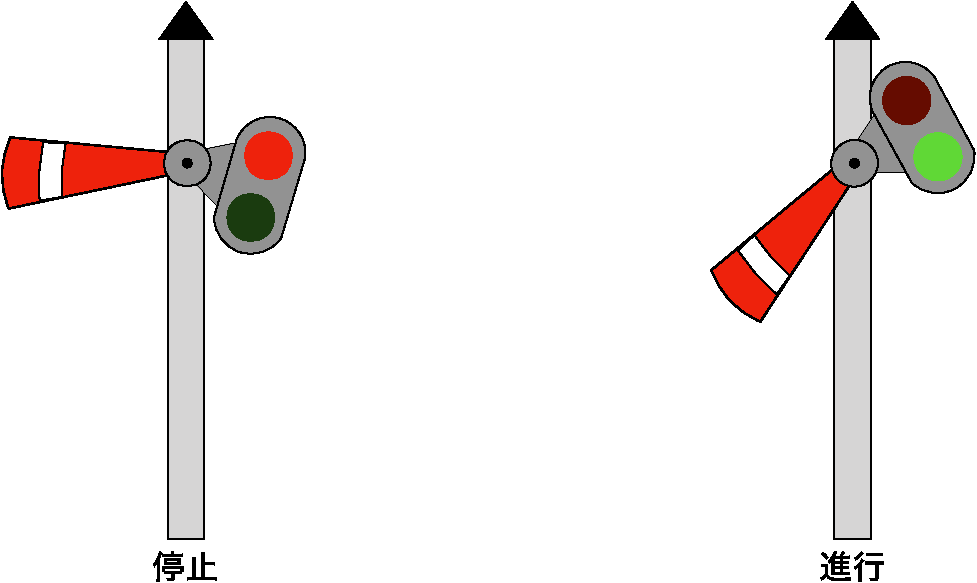
\includegraphics[scale=0.4]{Fig/semaphore-crop.pdf}
\end{myfig}

セマフォ型の変数は内部にカウンタ\footnote{
  腕木信号機の進行・停止のように二つの状態しか取らないものを
  \emph{バイナリセマフォと}呼ぶ.
  ここで取り上げるカウンタを持つものは\emph{カウンティングセマフォ}と呼ぶ.
  カウンタの値は0以上の整数値である.
}を持ち,また,プロセスの待ち行列を作ることができる.
セマフォ型(\|Sempahore|)の変数には,
\emph{P操作(Proberen:try)}と\emph{V操作(Verhogen:raise)}を
行うことができる.
カーネルはP操作とV操作を,
ユーザプロセスにシステムコールとして提供したり,
カーネル内部のサービスモジュールやデバイスドライバにサブルーチンとして提供したりする.
セマフォはプロセス(スレッド)の状態を\emph{待ち(Waiting)状態}に変える.
  \emph{ビジーウェイティングでは無い}のでCPUを無駄遣いすることはない.

\begin{quote}
  \begin{description}
  \item[P操作(P(S))]
    セマフォ(S)の値が1以上の場合は,セマフォの値を1減らす.
    そうでない場合は,プロセス(スレッド)を待ち(Waiting)状態にし,
    セマフォの待ち行列に追加する.
    アルゴリズムをC言語風に記述したものを\figref{semP}に示す.
  \item[V操作(V(S))]
    セマフォ(S)の待ち行列にプロセス(スレッド)がある場合は,
    それらの一つを起床させる.
    待っているプロセス(スレッド)が無い場合は,セマフォ(S)の値を1増やす.
    アルゴリズムをC言語風に記述したものを\figref{semV}に示す.
  \end{description}
\end{quote}

\begin{myfig}{btp}{セマフォのアルゴリズム}{semPV}
  \small\begin{center}
  \begin{minipage}{0.48\columnwidth}
    \lstinputlisting[numbers=none]{Lst/semP.c}
    \subcaption{P操作}
    \label{fig:semP}
  \end{minipage}\hspace{1em}
  \begin{minipage}{0.48\columnwidth}
    \lstinputlisting[numbers=none]{Lst/semV.c}
    \subcaption{V操作}
    \label{fig:semV}
  \end{minipage}
  \end{center}
\end{myfig}

\subsection{相互排除問題の解}
初期値が1のセマフォを用いて相互排除問題の解を示すことができる.
前出の架空の銀行口座管理プロセスの例を,
セマフォを用いて解決したものをリスト\ref{semMutex}に示す.

\lstinputlisting[numbers=left,float=btp,
  caption=セマフォを用いた相互排除問題の解,label=semMutex]{Lst/semMutex.c}

1行の\|account|は相互排除が必要なスレッド間の共有変数である.
2行の\|Semaphore|型の変数\|accSem|が排他制御に使用するセマフォである.
\|accSem|は1で初期化される.
クリティカルセクションに入るスレッドは,
まず,6行か14行で\|accSem|にP操作を行う.
どちらか先にやって来たスレッドがP操作を行った時点で\|accSem|の値が0になる.

遅れてやって来たスレッドは\|accSem|の値が0の間はクリティカルセクションに
入ることができない.
先のスレッドがクリティカルセクションを出て
8行か16行で\|accSem|にV操作を行ったら,
後のスレッドがクリティカルセクションに入ることができる.

\subsection{生産者と消費者問題(Producer-Consumer Problem)の解}
生産者スレッドはデータを生産し有限な長さの
\emph{リングバッファ(ring buffer)}に書き込む.
消費者スレッドはリングバッファからデータを読み出し消費する.
この時,満杯のリングバッファに更に書き込んだり,
空のリングバッファからデータを読み出したりしないように,
スレッド間で歩調を合わせる(同期する)必要がある.
セマフォを用いた解をリスト\ref{semProducerConsumer}に示す.

\lstinputlisting[numbers=left,float=btp,label=semProducerConsumer,
  caption=セマフォを用いた生産者消費者問題の解]{Lst/semProducerConsumer.c}

\begin{quote}
  \begin{description}
  \item [リングバッファとセマフォ]
    1行の\|buffer|は大きさ\|N|のリングバッファである.
    型は応用によって決まるので,リングバッファの型は仮に\|Data|型としている.
    2行の\|emptySem|はリングバッファの空きスロット数を表すセマフォである.
    最初は全てのスロットが空きなので初期値は\|N|である.
    3行の\|fullSem|はリングバッファの使用中スロット数を表すセマフォである.
    最初は使用中のスロットが無いので,初期値を 0 にしている.

  \item [生産者スレッド]
    4行から始まる\|producerThread|が,
    データを生産しリングバッファに書き込むスレッドである.
    5行の変数\|in|はリングバッファの次回書込み位置を表すローカル変数である.
    0,1,2,...,N-1,0,1,2,...の順に値が変化する.
    \texttt{in}はスレッドのローカル変数なので,
    \emph{相互排除をする必要がない.}

    \|producerThread|は,
    7行でデータを作り,
    8行で空きスロット数が1以上なら\|emptySem|の値を減らして,
    9行でデータをリングバッファに書き込む.
    10行で\|in|の値を更新している.
    11行で使用中スロット数\|fullSem|の値を増加させる.

  \item [消費者スレッド]
    14行から始まる\|consumerThread|は,
    データをリングバッファから読み出して消費するスレッドである.
    15行の変数\|out|はリングバッファの次回読出し位置を表すローカル変数である.
    \texttt{out}もスレッドのローカル変数なので,
    \emph{相互排除をする必要がない.}

    \|consumerThread|は,
    17行で空きスロット数が1以上なら\|fullSem|の値を減らして,
    18行でデータをリングバッファから読み出す.
    19行で\|out|の値を更新する.
    20行で空きスロット数\|emptySem|の値を増加させる.
    21行で読み出したデータを使用する.
  \end{description}
\end{quote}

\subsection{複数生産者と複数消費者問題(Producers-Consumers Problem)の解}
前の問題で,
関数\|producerThread()|,\|consumerThread()|それぞれについて,
複数のスレッドが存在する場合を考える.
バッファに関する同期の他に,
書き込み位置(\|in|),取出し位置(\|out|)に関する排他制御が必要になる.
解をリスト\ref{semMultiProducerConsumer}に示す.

\lstinputlisting[numbers=left,float=btp,,label=semMultiProducerConsumer,
  caption=セマフォを用いた複数生産者・複数消費者問題の解]
                {Lst/semMultiProducerConsumer.c}

\begin{quote}
  \begin{description}
  \item [リングバッファとセマフォ]
    1行から3行に変更はない.

  \item [生産者スレッド]
    次回書き込み位置を表す\|in|変数を
    複数の\|procucerThread|で共有する必要がある.
    \|in|変数の宣言を4行に移動し,スレッド間の共有変数に変更した.
    また,\|in|変数を\|procucerThread|間で相互排除するためのセマフォ\|inSem|を
    5行に追加した.

    \|producerThread|では,\|in|変数の参照や書き換えを行う11行と12行が
    \|in|変数に関するクリティカルセクションである.
    10行と13行に\|inSem|を用いた相互排除機構を追加した.

  \item [消費者スレッド]
    次回読み出し位置を表す\|out|変数について,
    生産者スレッドと同様な相互排除機構を追加してある.
  \end{description}
\end{quote}

\subsection{リーダ・ライタ問題(Readers-Writers Problem)の解}
\label{readersWritersProglem}
共有データに対して,
読み出し\emph{だけ}するリーダプロセス(スレッド)と,
読み出し書き込みの両方を行うライタプロセス(スレッド)の
二種類がある場合に,
単に資源をロックするより\emph{並行性(concurrency)}を高くすることができる.
リーダスレッドは,値を読み出すだけなので,
他のリーダスレッドと同時に共有データをアクセしても良い.
ライタスレッドは,値を書換えるので,
他のライタともリーダとも同時に共有データをアクセスすることは許されない.
セマフォによる解をリスト\ref{semReaderWriter}に示す.

\lstinputlisting[numbers=left,float=btp,label=semReaderWriter,
  caption=セマフォを用いたリーダ・ライタ問題の解]{Lst/semReaderWriter.c}

\begin{quote}
  \begin{description}
  \item [共有データとセマフォ]
    1行の\|records|が共有データである.
    2行の\|rwSem|は共有データの相互排除用のセマフォである.
    これらは,全てのスレッドに関係がある.

  \item [ライタスレッド]
    3行の\|writerThread|は共有データを書き換えることがあるスレッドである.
    書き換え途中に他のスレッドが共有データをアクセスすることを禁止するために,
    \|writerThread()|は6行で\|rwSem|にロックを掛ける.
    8行でロックを解除するまで,
    他のライタもリーダも同時に共有データにアクセスすることはできない.
    このようなロックを\emph{排他ロック(exclusive lock)}と呼ぶ.

  \item [リーダスレッド]
    13行の\|readerThread|は共有資源を読むことだけする.
    書き換え途中の不完全なデータを読み出さないように,
    \|writerThread|と相互排除を行う必要がある.
    しかし,書き換え途中以外なら,
    他のリーダスレッドと同時にデータを読んでも構わない.

    11行の\|cnt|変数はリーダスレッド間で共有される.
    12行の\|cntSem|セマフォは\|cnt|変数の相互排除用である.
    リーダスレッドはこれらを使用し,
    \|records|共有データを読み出し中のリーダスレッドの数を管理する.
    16行と17行,21行と22行の二箇所が,
    \|cnt|変数に関するクリティカルセクションである.

    16行では最初に読み出しを始めるリーダを判断し,
    最初のリーダだけが代表して\|rwSem|にロックを掛ける.
    二番目にやって来たリーダはロックを掛けないのでリーダ相互は排他されない.
    しかし,排他ロックを用いるライタとは相互排除される.
    このようなロックを\emph{共有ロック(shared lock)}と呼ぶ.
    22行で最後に読み出しを終えるリーダを判断し,
    最後のリーダだけが代表して\|rwSem|のロックを解除する.
  \end{description}
\end{quote}

リーダ・ライタ問題は,
共有ロックと排他ロックを使用する問題の例になっている.
共有ロックと排他ロックの考え方は,
ここに示したスレッド間の共有変数の管理だけでなく様々な場面で使用される.
例えばUNIXのシステムコールflockは,
引数に定数\|LOCK_SH|を渡すと共有ロックを,
定数\|LOCK_EX|を渡すと排他ロックをファイルに掛ける.
また,UNIXのopenシステムコールは,
引数に\|O_SHLOCK|フラグを指定すると共有ロックを,
引数に\|O_EXLOCK|フラグを指定すると排他ロックを,
ファイルのオープン時に自動的に掛ける.

%==============================================================================
\section{セマフォの実装例}
第\ref{tacosImpSemaphore}章に
TacOSにおけるセマフォの実装例を紹介する.
TacOSのセマフォはカウンティングセマフォである.
TacOSでは,
全てのプロセス間同期・排他はセマフォを使用して実現されている.

%==============================================================================
\section{まとめ}
この章ではプロセス間の同期に関係する話題を取り上げた.
\emph{クリティカルセクション}を実行する時は,
\emph{競合}が発生しないようにプロセス間の\emph{相互排除}をする必要がある.
オペレーティングシステムのカーネル内部などで,
短時間で終わるクリティカルセクションの相互排除を行う場合は,
\emph{割込み禁止}や\emph{専用命令}を\emph{ビジーウェイティング}と
組み合わせて使用する方法が使用できる.
専用命令としてTS命令,SW命令,CAS命令を紹介した.
CAS命令は\emph{ロックフリー}なアルゴリズムを実現するために使用できる.

クリティカルセクションの実行に長い時間がかかる場合は,セマフォなど,
プロセスの状態遷移を伴うオペレーティングシステムの機能を使用する.
セマフォを用いた\emph{相互排除問題}の解,
\emph{生産者と消費者問題}の解,
\emph{複数生産者と複数消費者問題}の解,
\emph{リーダ・ライタ問題}の解を学んだ.

%==============================================================================
\section*{練習問題}
\begin{enumerate}
  \renewcommand{\labelenumi}{\ttfamily\arabic{chapter}.\arabic{enumi}}
  \setlength{\leftskip}{1em}
\item 次の言葉の意味を説明しなさい.
  \begin{enumerate}
  \item 競合
  \item クリティカルセクション
  \item 相互排除
  \item ビジーウェイティング
  \item ロックフリーなアルゴリズム
  \item セマフォ
  \item 相互排除問題
  \item 生産者と消費者問題
  \item リーダライタ問題
  \end{enumerate}
\item なぜ割込みを禁止することで相互排除ができるか?
\item 割込み禁止による相互排除がマルチプロセッサシステムでは
  不十分な理由は?
\item 割込み禁止による相互排除はクリティカルセクションの三つの条件を
  満たしているか?
\item CPUが割込み禁止になっている間に発生した割込みはどのように
  扱われるか?
\item DI命令やEI命令が特権命令でなかったら,どのような不都合が生じるか?
\item シングルプロセッサシステムにおいて,
  機械語命令は\emph{アトミック(atomic)}と言えるか?
\item マルチプロセッサシステムにおいて,
  機械語命令は\emph{アトミック(atomic)}と言えるか?
\item TS命令とSW命令に共通な特長は何か?
\item \figref{testAndSet}のようなビジーウェイティングは
  シングルプロセッサシステムでも使用できるか?
\item セマフォを相互排除に使用する手順を説明しなさい.
\item 生産者と消費者の問題において,
  二つのセマフォはどのような値に初期化されたか?\\
  二つのセマフォは何の役割を持っていたか?
\end{enumerate}
